\section{Design development - hardware}

\subsection{System Architecture}
Overall system architecture is outlined in Figure~\ref{flow:system_architecture}, each individual subsystem will be outlined in detail the following sections.
\tikzstyle{block} = [rectangle, draw, fill=\myblue, 
    text width=5em, text badly centered, rounded corners, minimum height=4em]
\tikzstyle{line} = [draw, -latex']
\begin{figure}[H]
\centering
\fbox{
\begin{tikzpicture}[node distance = 1.85cm]
\node [block, fill=\myorange] (cuk) {DC-DC converter};
\node [block, below = of cuk, fill=\myblue] (load) {load};
\node [block, right = of cuk, fill=\myblue] (drivers) {gate drivers};
\node [block, above = of cuk, fill=\myblue] (sensingoutput) {output voltage sensing};
\node [block, above = of sensingoutput, fill=\myblue] (sensinginput) {input voltage sensing};
\node [block, above left = of sensinginput, fill=\myblue] (charging) {charging circuitry};
\node [block, below = of charging, fill=\myblue] (caps) {ultra-capacitors};
\node [block, right = of drivers, fill = \mygreen] (PWM) {PWM};
\node [block, above right = of sensinginput, fill=\myblue] (USB) {USB};
\node [block, right = of sensingoutput, fill = \mygreen] (ADC) {ADC};
\node [block, right = of ADC, fill = \mygreen] (uC) {micro-controller};
\node [block, right = of USB, fill=\myblue] (UART) {UART};
%
\path [line, ultra thick] (USB)	-- node [anchor = south, align = center] {power} (charging);
\path [line, ultra thick] (charging) to[out = -90, in = 90] node [anchor = east, align = center]
	{power}	(caps);
\path [line, ultra thick] (caps) to[out = -90, in = 180] node [anchor = west, align = center]
	{$v_g$}	(cuk);
\path [line, ultra thick] (cuk)	--	node [anchor = west, align = center] {$y$} (load); 
\path [line, ultra thick] (USB)	to[out = -90, in = 150]	node [anchor = west, align = center]
	{power}	(uC);
\path [line, ultra thick] (USB)	to[out = -40, in = -140] node [anchor = south, align = center]
	{\textsf{ref}} (UART);
\path [line, ultra thick] (UART) to[out = -110, in = 110] node [anchor = west, align = center]
	{\textsf{ref}} (uC);
\path [line, ultra thick] (caps) to[out = 0, in = -180]
	node [anchor = south, align = center, above left = 0cm and -0.25cm]	{$v_g$}	(sensinginput);
\path [line, ultra thick] (cuk)	to[out = 90, in = -90] node [anchor = west, align = center]
	{$y$} (sensingoutput);
\path [line, ultra thick] (uC) to[out = 70, in = -70] node [anchor = west, align = center]
	{measurements; \\ estimates} (UART);
\path [line, ultra thick] (uC) to[out = -90, in = 90] node [anchor = west, align = center]
	{$d$} (PWM);
\path [line, ultra thick] (UART) to[out = 140, in = 40]	node [anchor = south, align = center]
	{measurements; \\ estimates} (USB);
\path [line, ultra thick] (PWM)	-- node [anchor = north, align = center] {switching \\ signal}
	(drivers);
\path [line, ultra thick] (drivers)	--	node [anchor = north, align = center] {switching \\ signal}
	(cuk);
\path [line, ultra thick] (ADC) -- node [anchor = north, align = center] {measured \\ voltages}
	(uC);
\path [line, ultra thick] (sensinginput) to[out = -20, in = 110]
    node [anchor = south, align = center, above right = 0.75cm and -1.5cm] {$v_g$ \\ (filtered)}
	(ADC);
\path [line, ultra thick] (sensingoutput) -- node [anchor = north, align = center]
    {$y$ \\ (filtered)} (ADC);
\end{tikzpicture}
}
\caption{}
\label{flow:system_architecture}
\end{figure}
%%%%%%%%%%%%%%%%%%%%%%%%%%%%%%%%%%%%%%%%%%%%%%%%%%%%%%%%%%%%%%%%%%%%%%%%%%%%%%%%

%%%%%%%%%%%%%%%%%%%%%%%%%%%%%%%%%%%%%%%%%%%%%%%%%%%%%%%%%%%%%%%%%%%%%%%%%%%%%%%%
\subsection{Microcontroller}
To implement the controller digitally an microcontroller (MCU) was required to carry out the computations. In addition to interfacing with external peripheral circuitry, the MCU has four main responsibilities that include:
\begin{itemize}
    \item Measurement of the input and output voltages of the \'Cuk Converter.
    \item Calculation of control action.
    \item Generating switching signal for the converter.
    \item Communication with host machine.
\end{itemize}
The calculations required for the control algorithm are computationally expensive and must be executed online (that is computed in real time rather than pre-computed offline). This type of computation is well suited to a digital signal processors (DSP).
\\ \\
The MCU was carefully chosen such that as many of the critical components were included as peripherals rather than requiring external components. This saved board space and allowed for a less complicated design, it also saved time as it removed the need to interface with the components using serial communication protocols. The main peripherals required were a fast ADC at a high resolution in addition to DAC that supported PWM at the high frequencies to allow for smaller components.
\\ \\
Microchip's dsPIC33EP ``GS'' series of specialised digital signal controllers are designed for high-speed digital control loops and contained the additional peripherals for interfacing with external circuitry. Specifically the \texttt{dsPIC33EP64GS504} was chosen, as it also contained a number of peripherals tailed for switched mode power supply control.
\begin{figure}
    \centering
    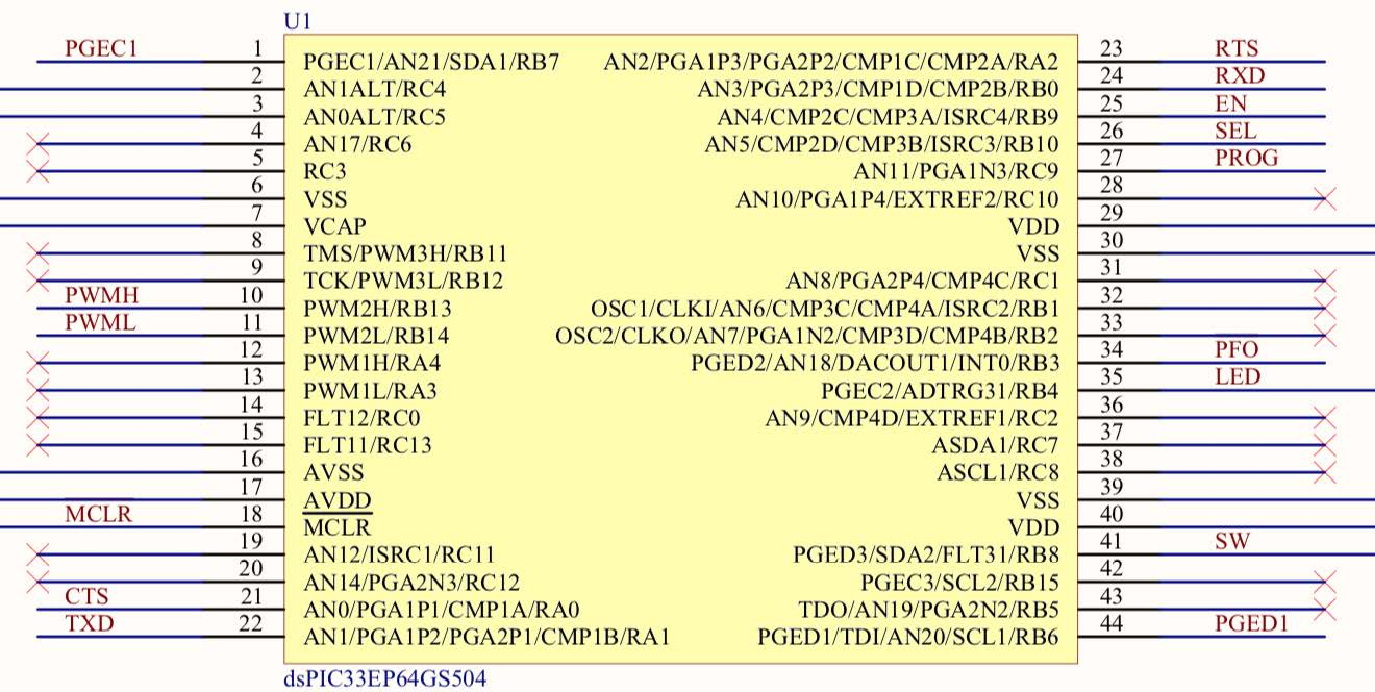
\includegraphics[height = 8cm]{figures/hardware/mcu_schematic.pdf}
    \caption{MCU schematic excerpt.}
    \label{fig:mcu_schematic}
\end{figure}
Operating at a clock rate of \SI{120}{MHz}, the MCU is capable of \SI{60}{MIPS}. This is generated using the internal fast RC oscillator (FRC) that provides a nominal \SI{7.37}{MHz} clock. As this is a RC oscillator, timer accuracy would be limited and affected by a number of external factors (such as temperature). However as the sampling rate was chosen to be \SI{10}{kHz} (section \ref{sec:system_params}) the presence of jitter proved not to affect the performance of the converter. An external clock could be used for addition precision, it was decided to avoid including this in the initial design as it would complicated the PCB layout as well and increasing the time required to write firmware for the device.
%%%%%%%%%%%%%%%%%%%%%%%%%%%%%%%%%%%%%%%%%%%%%%%%%%%%%%%%%%%%%%%%%%%%%%%%%%%%%%%%
\subsubsection{Analog-to-digital converter (ADC)}
The \texttt{dsPIC33EP64GS504} contained an high-speed ADC module was several desirable features:
\begin{itemize}
    \item Four dedicated SAR cores each configurable for up to 12-bits of resolution. This feature was central in the choice of the micro controller as it allowed for the simultaneous measurements of all four of the \'Cuk converter states if observer implementation proved to be difficult or the execution speed was too slow.
    \item Up to 3.25 Msps conversion rate per channel at 12-bit resolution, when using a \SI{70}{MHz} instruction clock.
    \item Flexible and independent ADC trigger sources that allow for minimal CPU interaction, allowing the ADC to run independently while the costly control algorithm is computed.
\end{itemize}

\paragraph{Successive approximation register (SAR) ADC}
Conversion of the continuous analog signal into a discrete digital representation occurs via a binary search. Through the use of a digital-to-analog converter the ADC generates a reference voltage and compares it to the analog voltage that was sampled. For each of the 16-bits of digital data (starting with the most significant bit) the SAR compares if the voltage is higher or lower than the voltage generated by the data, eventually converging on the final quantisation level and generating the 16-bit digital word \cite{sar_adc}.
\\ \\
SAR ADCs are inherently slow due to the nature of the algorithm that they implement, as the algorithm must narrow in on the voltage over a number of stages that scales with the number of bits used in the representation. The rate at which conversions occur is directly coupled to the instruction clock. For maximum conversion rate the instruction clock should be configured to be as high as possible. For ideal performance the ADC must convert the signal instantaneously at the start of the sampling interval. To approximate this the conversion time should be approximately an order of magnitude smaller than the sampling period. Since \SI{10}{kHz} was chosen for the sampling rate, and a \SI{60}{MHz} instruction clock was used, the ADC conversion rate is 620ns. This is much smaller than the sampling period of 20us and hence approximately occurred instantaneously.
%%%%%%%%%%%%%%%%%%%%%%%%%%%%%%%%%%%%%%%%%%%%%%%%%%%%%%%%%%%%%%%%%%%%%%%%%%%%%%%%
\subsubsection{Pulse width modulation (PWM)}
A single fast PWM module was sued to send switching signal to the DC-DC converter. PWM signal was configured to run at \SI{10}{kHz} and duty cycle is controlled by writing to a register, PDC1. 
%%%%%%%%%%%%%%%%%%%%%%%%%%%%%%%%%%%%%%%%%%%%%%%%%%%%%%%%%%%%%%%%%%%%%%%%%%%%%%%%
\subsubsection{Timer}
A single 16-bit timer module was used to implement the sampling rate of converter. ADC triggering was against this timer to ensure sampling occurred at the start of each interval. Controller computations were also executed within this sampling period.

\subsubsection{Programmer}
An in-circuit serial programmer (ICSP) was used for debugging and flashing of microcontroller firmware. The Microchip \textit{PICkit\textsuperscript{TM} 3 In-Circuit Debugger} was untilised and require six connections via a standard header on the PCB, see appendix \ref{apn:pcb}.
%%%%%%%%%%%%%%%%%%%%%%%%%%%%%%%%%%%%%%%%%%%%%%%%%%%%%%%%%%%%%%%%%%%%%%%%%%%%%%%%
\newpage
\subsection{USB Interface}
A USB Interface was included to serve two purposes:
\begin{itemize}
    \item Primary source of power to the system, supplying up to \SI{500}{mA} of current to charge the ultra-capacitors.
    \item Communication with the host machine; providing serial output for firmware debugging as well as controller configuration.
\end{itemize}

This was quickly extended to be the main port of control, as the device was to be powered via the USB port of a computer, also being able to configure the device (i.e set reference point) over USB was the natural next step. Doing so avoid the need to a design a hardware interface for controlling the device, which would have required a display and other peripherals. It was also likely that that control algorithms would be costly and therefore leave very little computation time for displaying graphics on an LCD display incorportated into the device.
%%%%%%%%%%%%%%%%%%%%%%%%%%%%%%%%%%%%%%%%%%%%%%%%%%%%%%%%%%%%%%%%%%%%%%%%%%%%%%%%

\subsubsection{USB to serial}
The FTDI FT232R USB to serial UART interface implements the USB protocol on a single chip, offloading the processing from the main microcontroller. This chip incorporates the high speed termination resistors and clock to further simplify the design \cite{ft232r}.
\begin{figure}
    \centering
    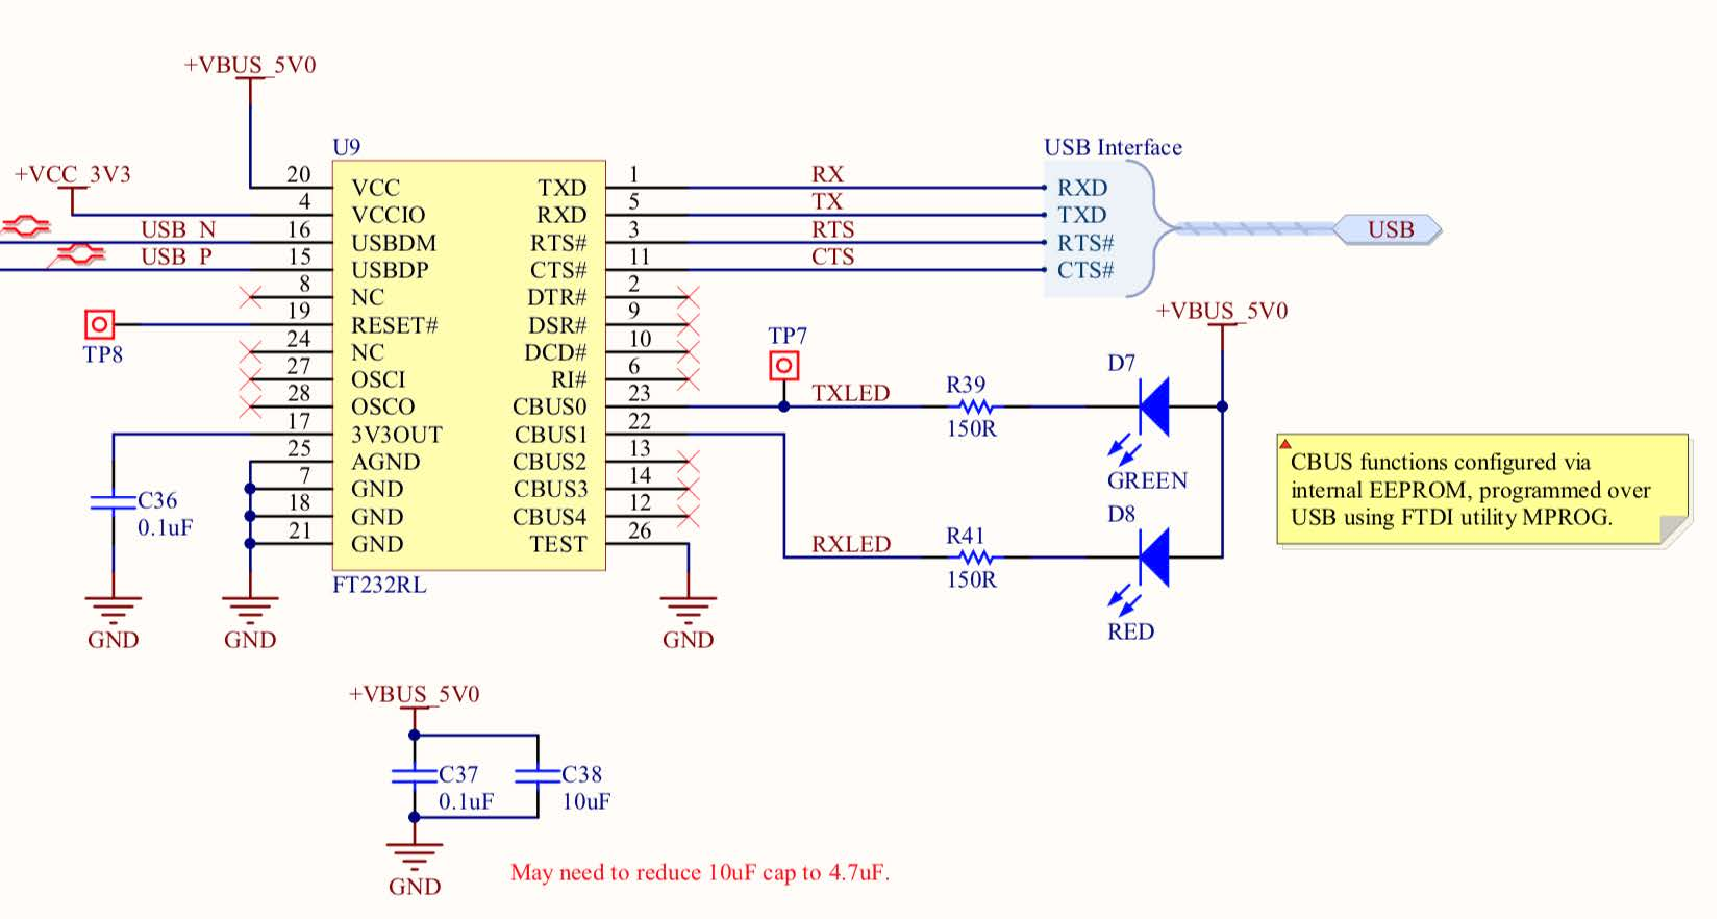
\includegraphics[height = 8cm]{figures/hardware/usb_schematic.pdf}
    \caption{USB schematic excerpt.}
    \label{fig:usb_schematic}
\end{figure}
To communicate with the MCU via UART requires two physical connections: one to receive data (RX) and one to transmit data (TX). These are connected to the opposite pins on each device. In the first prototype additional hand-shaking connections were included (RTS and CTS) in case they were required. Since each device were operating at similar rates to each other, that is they processes the data received via UART at similar rates, they did not require hand-shaking to add artificial wait time in between transmissions so one of the devices could wait for the other before transmitting the next byte. This ensure that data is not lost during the transmission process. 
\\ \\
Status LEDs were connected via current limiting resistors to the CBUS0 and CBUS1 pins of the FT232R. This allowed for visual feedback to confirm when data was being received and transmitted to the chip over UART, allowing for a simple check rather than having to connect and configure an oscilloscope or logic analyser each time.
\begin{itemize}
    \item The CBUS pins can be configured for a number of functions, one option sets the pins to be used as LED drivers for received/transmitted data. This is conveniently the default configuration of the device, which avoided having to externally program the EEPROM using software utility provided by the manufacturer (FTDI).
    \item Feature proved useful during debugging on a number of occasions.
\end{itemize}

It was important to ensure that \texttt{VCCIO} was connected to the same supply as the MCU, in this case \SI{3.3}{V}. In in the initial prototype this was connected to the MCU \SI{3.3}{V} voltage rail, which lead to some minor issues detailed below. In the final revision this pin was connected directly to the \texttt{3V3OUT} pin and hence uses the internal LDO regulator to supply the reference, this is the option recommended in the datasheet \cite{ft232r} and also improved the layout of the PCB (separated power rails, reduced noise that would couple off the line).

%%%%%%%%%%%%%%%%%%%%%%%%%%%%%%%%%%%%%%%%%%%%%%%%%%%%%%%%%%%%%%%%%%%%%%%%%%%%%%%%

\subsubsection{Power filtering and input protection}
Following the USB Hardware Design Guidelines \cite{usb_design_guide} recommends that a \SI{10}{nF} capacitor and a ferrite bead should be placed as close to the USB connector as possible. The ferrite bead in conduction with the capacitors in a PI configuration form an LC filter that helps to smooth the USB power supply \cite{usb_filtering}.
\begin{figure}
    \centering
    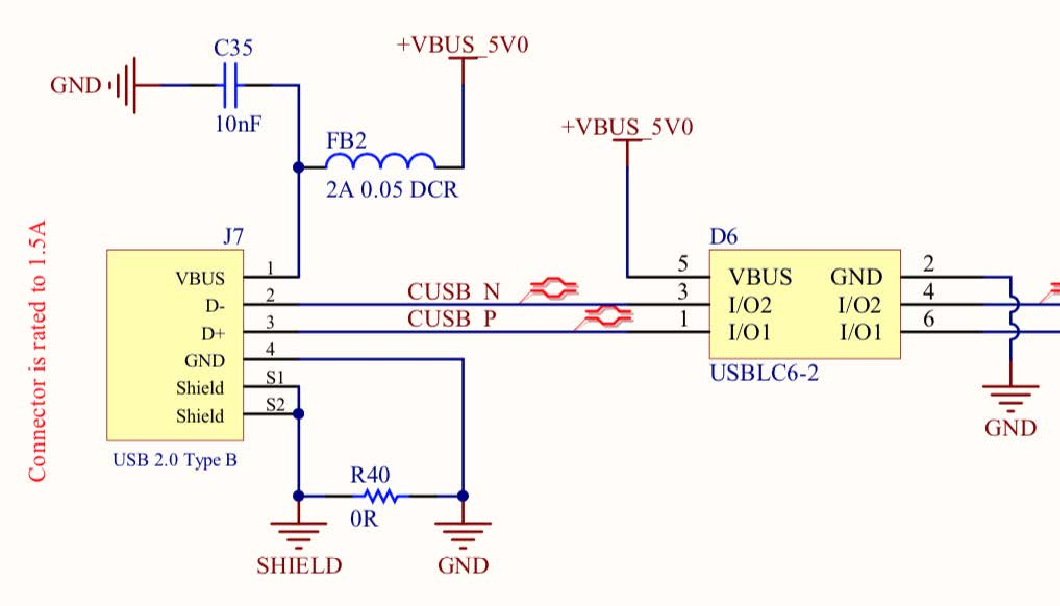
\includegraphics[height = 8cm]{figures/hardware/usb_power.pdf}
    \caption{USB power filtering and protection schematic excerpt.}
    \label{fig:usb_power}
\end{figure}
As shown in figure \ref{fig:usb_power}, a zero-ohm resistor was included between the shield and ground as the shield of a USB cable acts as an antenna. As such connecting the shield directly to the signal ground on the PCB should be avoided. In the case that EMI becomes and issues the zero-ohm resistor could be replaced with an inductor/ferrite bead.
\\ \\
Transient-voltage-suppressot (TVS) diodes are place as the first device next to the external USB connector to provide the shortest current path to ground in the case of an electrostatic discharge event were to occur. This minimises the possibility of damage elsewhere on the PCB.
%%%%%%%%%%%%%%%%%%%%%%%%%%%%%%%%%%%%%%%%%%%%%%%%%%%%%%%%%%%%%%%%%%%%%%%%%%%%%%%%
%%%%%%%%%%%%%%%%%%%%%%%%%%%%%%%%%%%%%%%%%%%%%%%%%%%%%%%%%%%%%%%%%%%%%%%%%%%%%%%%
\newpage
\subsection{Sensing}
As the controller required the simultaneous measurement of both the input and output voltages it was important to condition the signals to appropriate levels such that they could be sampled by correctly by the ADC.
\tikzstyle{block} = [rectangle, draw, fill=\myblue, 
    text width=6em, text badly centered, rounded corners, minimum height=4em]
\begin{figure}[H]
\centering
\fbox{
\begin{tikzpicture}[node distance = 1cm]
\node [block, fill=\myblue, text width=4em] (scaling) {scaling};
\node [block, right = of scaling, fill=\myblue, text width=5em] (buffering) {buffering};
\node [block, right = of buffering, fill=\myblue, text width=5em] (gainstage) {gain stage};
\node [block, right = of gainstage, fill=\myblue, text width=6em] (antialiasing) {anti-aliasing};
\node [block, right = of antialiasing, fill=\myblue, text width=5em] (clamping) {clamping};
%
\path [line, ultra thick] (scaling)	-- (buffering);
\path [line, ultra thick] (buffering) -- (gainstage);
\path [line, ultra thick] (gainstage) -- (antialiasing);
\path [line, ultra thick] (antialiasing) -- (clamping);
\end{tikzpicture}
}
\caption{Voltage sensing system architecture.}
\label{fig:sensing_system}
\end{figure}
The expected voltages and frequency content of the input and output are different and hence need to be designed separately. Both signals must past through five stages (see figure \ref{fig:sensing_system}) before they are appropriate to be sampled by the ADC; each stage will be outlined in detail below. First, we must outline the characteristics of the two signals that we wish to measure.

\paragraph{Input voltage}
The input of the \'Cuk Converter is directly connected to the top of the ultra-capacitor stack. Hence, we can expect a slowly varying signal that is between \SI{0}{V} and \SI{5}{V}. The frequency content of this voltage will be low frequency and hence a low order passive anti-aliasing filter will be appropriate. It should also be noted that this signal if positive with respect to ground and hence will not require inversion.
\begin{figure}[H]
    \centering
    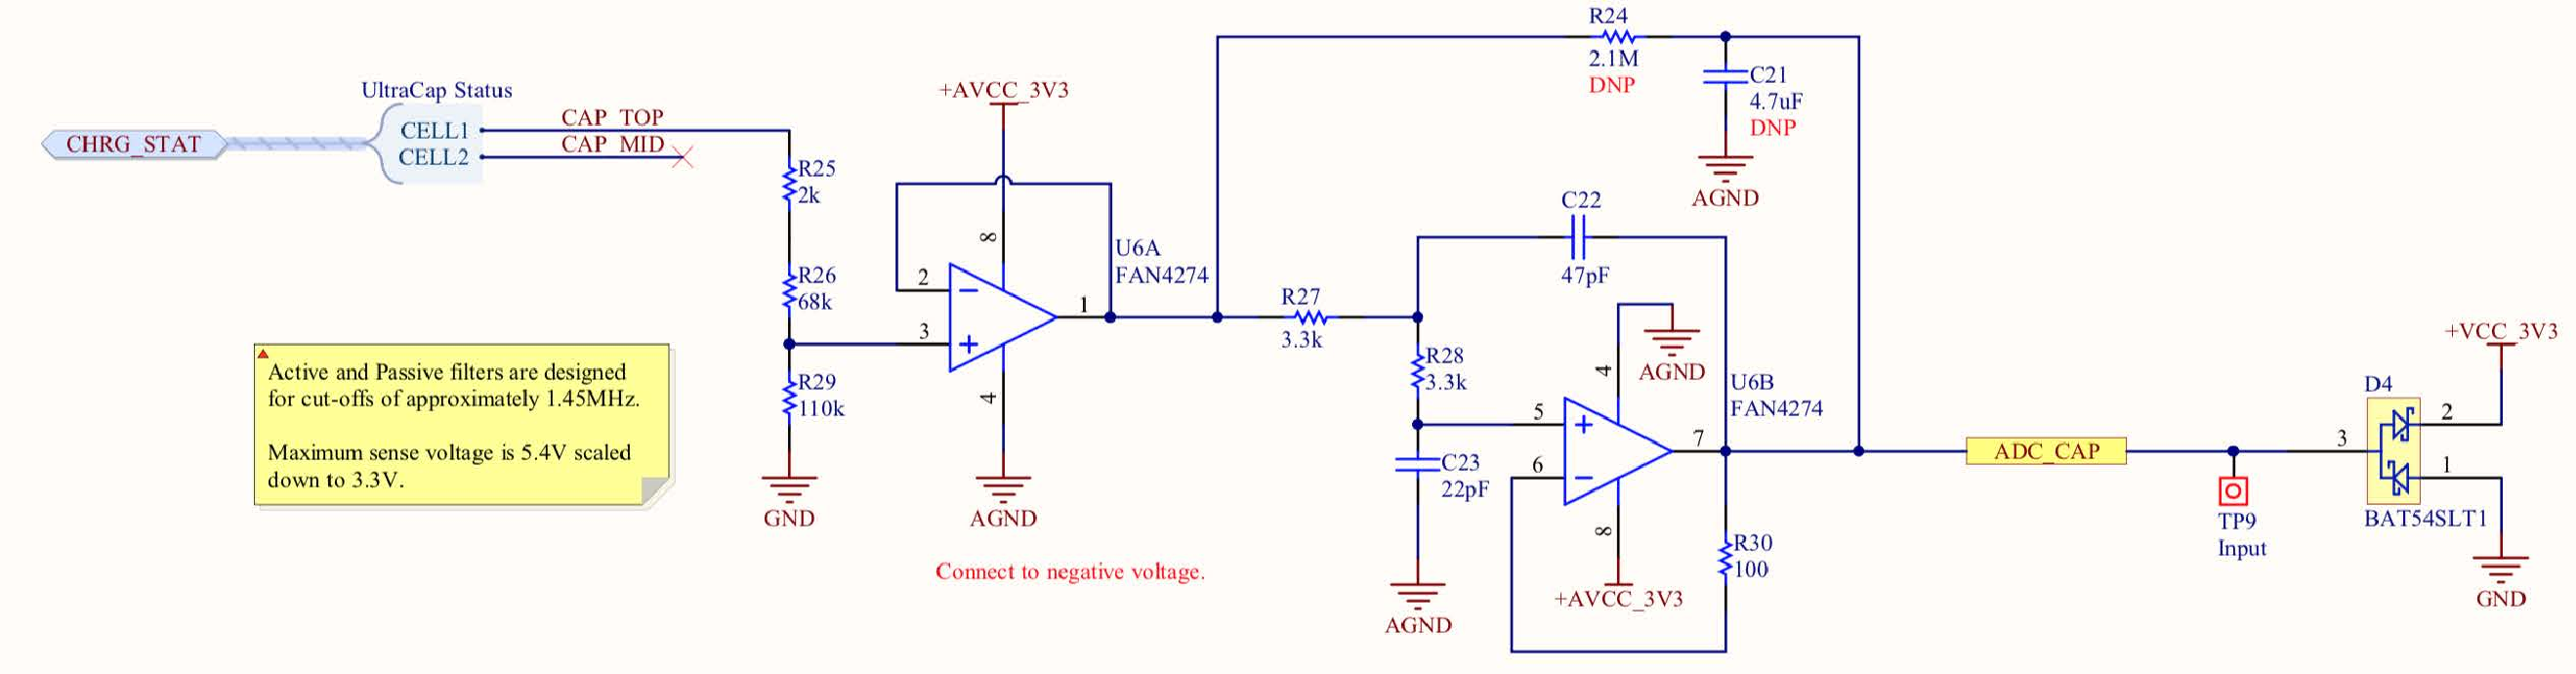
\includegraphics[width = 14cm]{figures/hardware/input_sense.pdf}
    \caption{Converter input voltage schematic excerpt.}
    \label{fig:input_sense}
\end{figure}

\paragraph{Output voltage}
The output of the \'Cuk Conveter is significantly more complicated than the input. It contains high frequency switching content from the MOSFET switching at a nominal \SI{100}{kHz} and will also contain fast transient due to the control action. It is vital that this information is preserved for optimal performance of the controller. To preserve as much of the high frequency we must use a higher order active filter with a smaller transition region around the Nyquist frequency.

As the \'Cuk Converter topology produces an inverted output voltage with respect to ground, care must be taken to invert this signal such that it can be sampled correctly by the ADC. The MCU contains a rail-to-rail analog to digital converter (ADC) and hence can sample voltages between 0 and \SI{3}{V} (positive). Hence a gain stage must include a negative gain such that the voltage is positive. As theoretically the output of the converter can be anything that we choose it to be, it was decided to specify and support output voltages between $-\SI{15}{V}$ and \SI{0}{V}.
\begin{figure}[H]
    \centering
    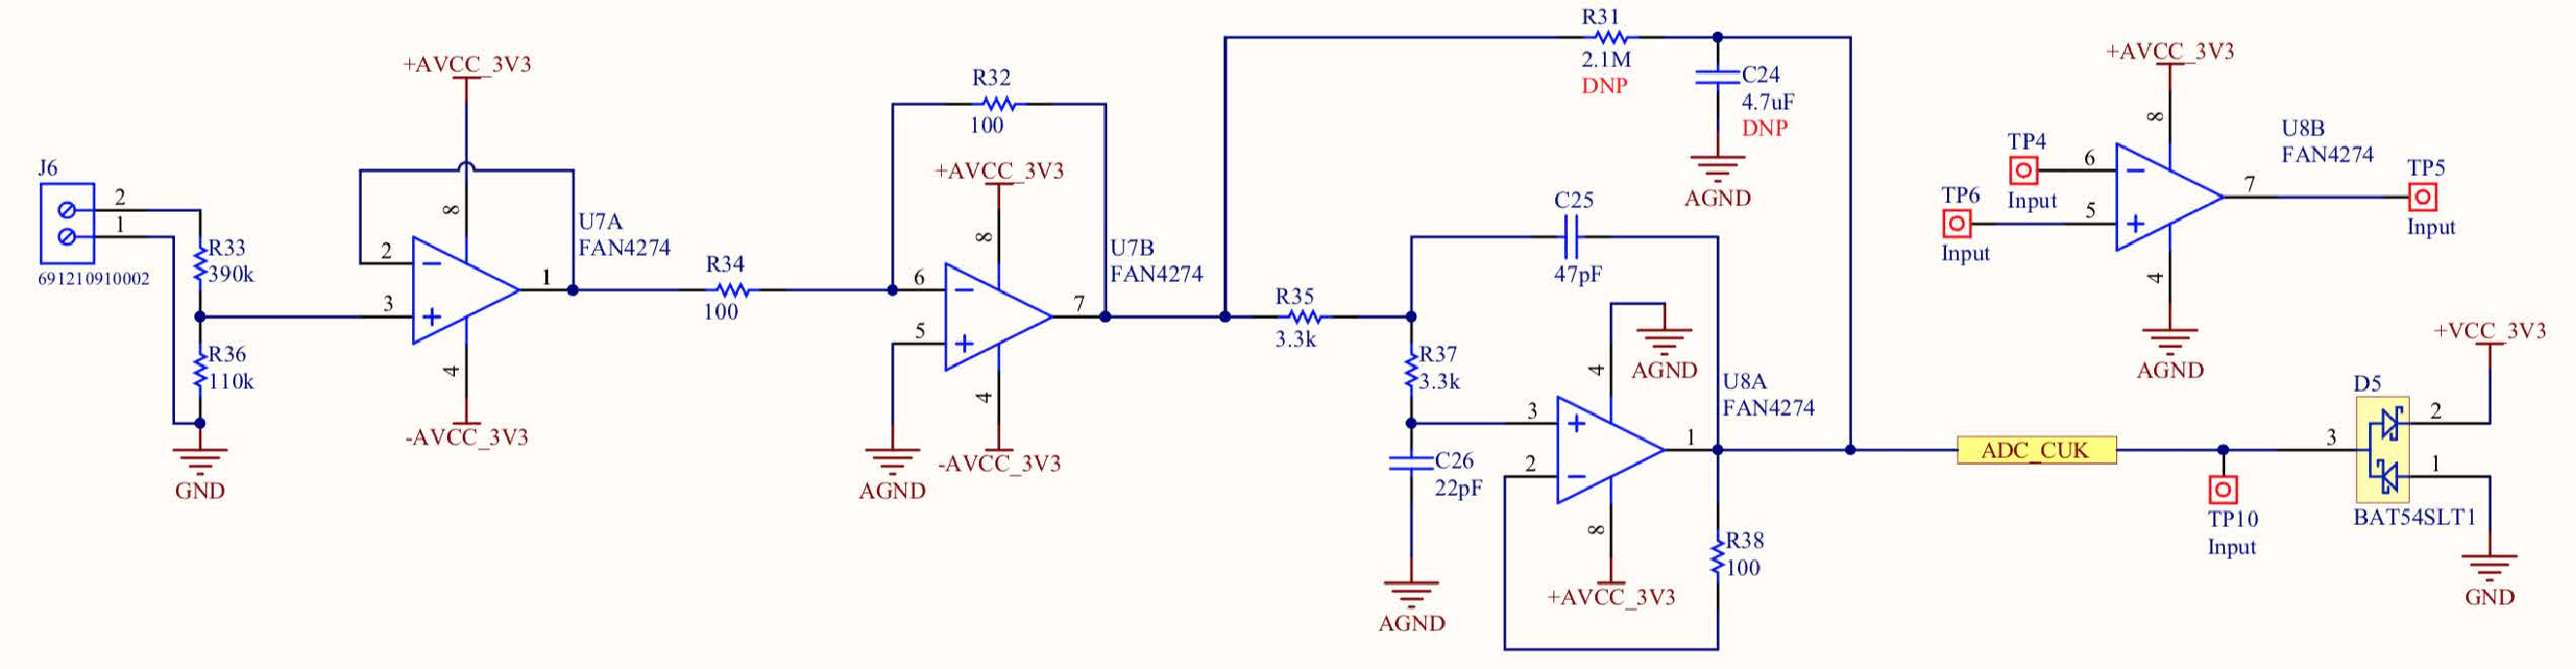
\includegraphics[width = 14cm]{figures/hardware/output_sense.pdf}
    \caption{Converter output voltage schematic excerpt.}
    \label{fig:output_sense}
\end{figure}

\subsubsection{Scaling}
As the chosen microcontroller can only sample voltages from \SI{0}{V} to \SI{3.3}{V}, we must scale the voltage of both the input and output such that the voltage is between these stages. To ensure maximum resolution of the sampled voltage and avoid quantisation from affecting the measurements it was important to ensure that the voltages could swing between the \SI{0}{V} and \SI{3.3}{V} range without experiencing clipping. To achieve this a resistive divider was employed to scale the voltage down by a set factor.
\\ \\
In order to reduce power loses the quiescent current must be traded off with the loading of the operation amplifier. Using too low of a resistance for the divider would result in high quiescent currents and hence large power loses, too high of a resistance would being to be loaded by the operational amplifier. As the input impedance of an operational amplifier is unknown and varies significantly between devices, by design, we are unable to compensate for the loading and thereby the accuracy of the measurements will be affected. We found that choosing resistors in the \SI{100}{k\ohm} range performed well. It was also essential that low tolerance ($\pm0.1 \%$) resistances were chosen such that accuracy could be maintained.
\\ \\
Once the voltages were scaled, they would be re-scaled inside the microcontroller by multiplying by a constant factor that divided on the resistors used in the voltage divider. If these resistances themselves where not known to a high degree of accuracy this scaling factor would be significantly out of specification.

\subsubsection{Buffer}
So that the voltage divider was not loaded by the filter stage and affecting the accuracy of the results. The resistances of the filters were chosen to be of a similar order of magnitude to the resistive divider to avoid current saturation of the operational amplifiers and to minimise power losses, hence loading was a real concern.
\\ \\
By including an operational amplifier configured as a buffer the high impedance input and low impendence output would avoid loading of either stage.


\subsubsection{Gain Stage}
As the output voltage of the \'Cuk converter is negative an operational amplifier configured as a unity gain inverting amplifier was required.

%Initially the resistances chosen for the feedback weas too small resulting in current saturation of the op amp. Too much current was being drawn from the buffer stage causing the voltage to saturate around 2.2V.

\subsubsection{Anti-aliasing filter}
The input and the output of the DC-DC converter must pass through an anti-aliasing filter such that any high frequency content is removed before the signal is sampled by the ADC. Failure to remove this high-frequency noise results in folding and will corrupt the low frequency content. Since the output has a lot of high frequency content, ripple and transients that should be measured it is important that the AA filter has a fast roll off to ensure as much of this signal is preserved as possible. For the input, this isn’t as important. It is slowly varying, hence a first order passive filter was employed instead.
\\ \\
``A practical anti-aliasing filter should have a magnitude response approximately unity in the passband, a stopband response exceeding a minimum attenuation level and an acceptable transistion band separating the passband and stopband.'' \cite{dsp} A butterworth low pass filter meets these requires and was designed using the Sallen Key topology for a cut-off at Nyquist rate \SI{5}{kHz}. The topology and component values are shown in figure \ref{fig:output_sense}.

\subsubsection{Clamping}
To ensure the pins of the microcontroller and not destroyed by exceeding their maximum voltage rating, diodes were employed to clamp the voltages to within a fixed range. If a voltage exceed \SI{3.3}{V} plus the forward voltage of the diode, the diode would appear as a short circuit to the signal and hence any potentially damaging voltages would appear across the diodes rather than the microcontroller pins.

\subsubsection{Operation amplifier}
The main deciding factor for operational amplifier with a large gain bandwidth product. This was due to a the sampling frequency being unspecified while the control algorithm was being designed and also to due to a lack of understanding in regards to how high frequency content affect the performance of the controller. Hence an operational amplifier was chosen such that it exceeds the half the maximum sampling rate of the ADC.
\\ \\
The FAN4274 from ON Semiconductor provided the performance we required while also offering dual operational amplifiers in the single package, reducing board space \cite{fan4274}.
\\ \\
Despite having a \SI{5}{V} rail, the operational amplifiers were supplied by $\pm\SI{3.3}{V}$ as the $\pm{5}{V}$ would not provide any extra resolution to the ADC and simply result in additional power losses.
%%%%%%%%%%%%%%%%%%%%%%%%%%%%%%%%%%%%%%%%%%%%%%%%%%%%%%%%%%%%%%%%%%%%%%%%%%%%%%%%
\newpage
\subsection{Charging circuitry}
The LTC4425 is designed to charge a two ultra-capacitors in series from a USB port , forming a stack. It incorporates internal voltage clamp circuity to two present voltages, \SI{2.45}{V} or \SI{2.7}{V}, to prevent either of the ultra-capacitors from exceeding their maximum rated voltage. This clamping voltage can be configured externally and allowed flexibility for the ultra-capacitors chosen. It also allowed for an extra margin of safety for the \SI{2.7}{V} rated ultra-capacitors that were eventually chosen for the final design.
\\ \\
It was decided early on in the design process that a dedicated ultra-capacitor charge chip would be used rather than designing our own charging circuit using discrete components. This would free up a considerable amount of time that could then be used to design the rest of the hardware and fine tune the control algorithm.
\begin{figure}
    \centering
    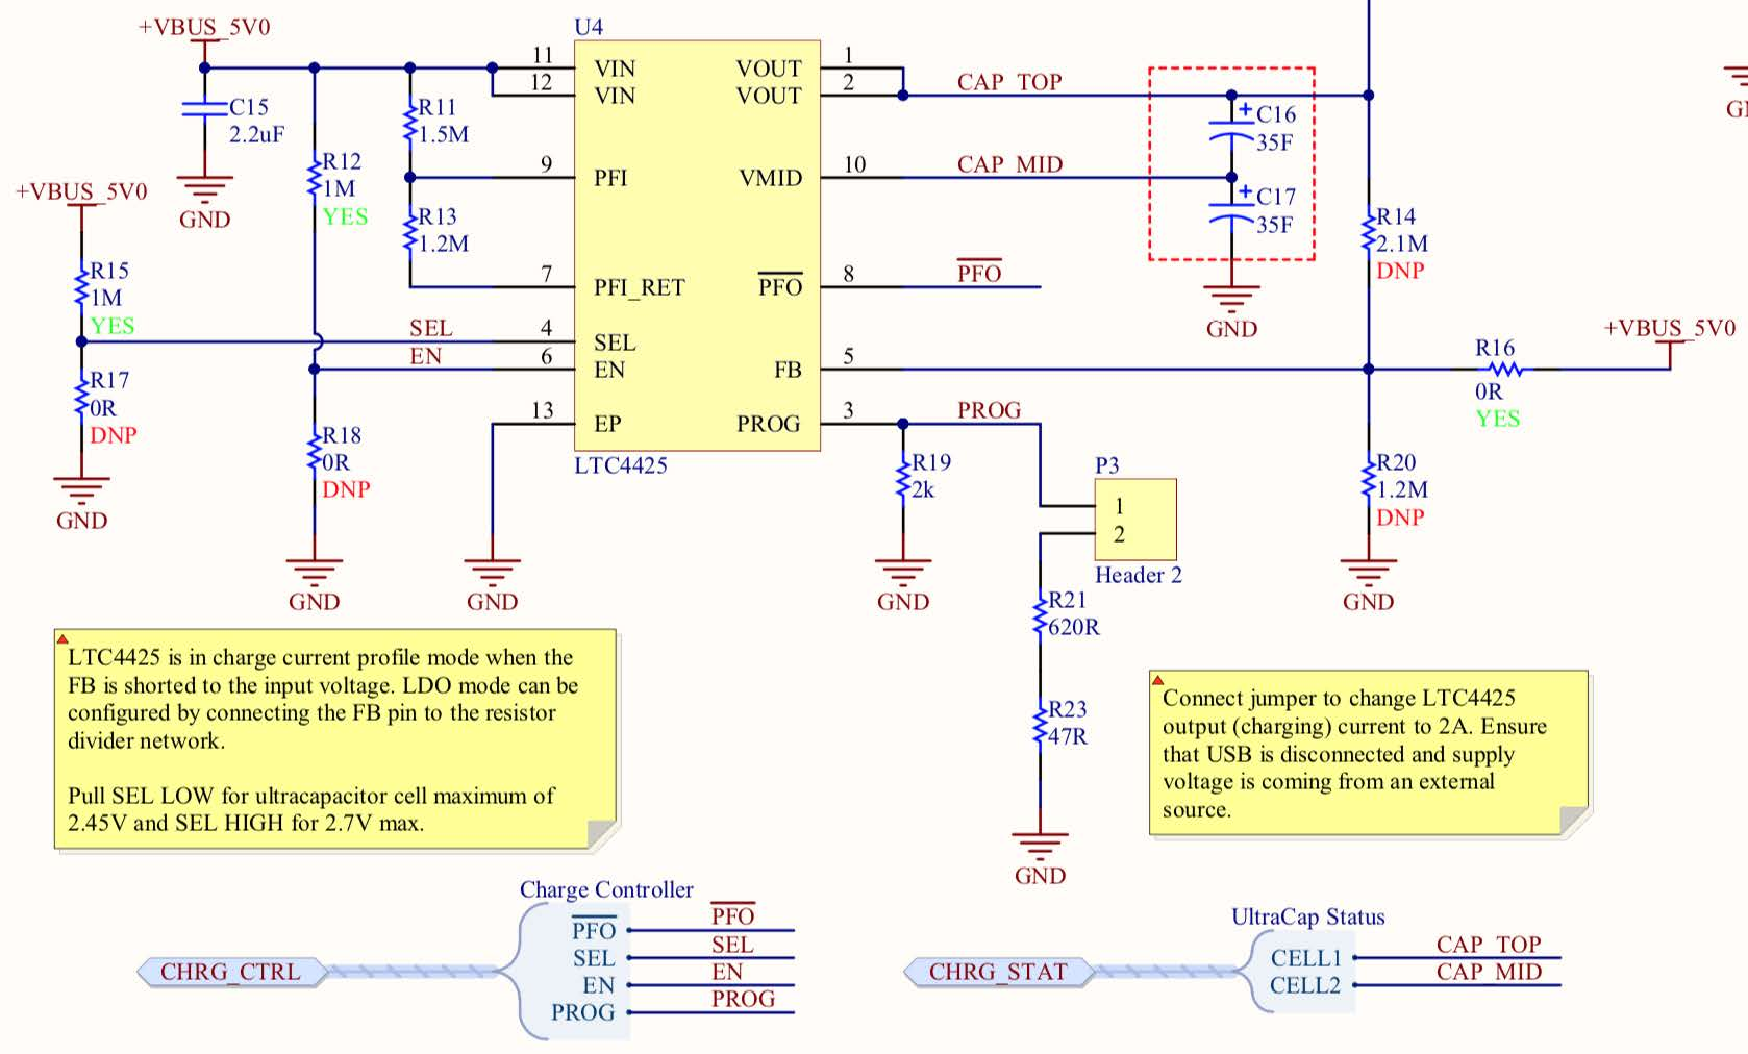
\includegraphics[height = 10cm]{figures/hardware/charging_schematic.pdf}
    \caption{Ultra-capacitor charging schematic excerpt.}
    \label{fig:charging}
\end{figure}
As capacitors appear as shorts to source voltages appearing across them that are higher than there currently stored voltage. Due to manufacturing tolerances the internal ESR of the capacitors can vary, this can lead to one of the capacitors sinking all the current, which causing one of the capacitors in the series stack to charge fully while the other does not. As the cell stack is being charged to \SI{5}{V} if one of the ultra-capacitors were to dominate it will lead to that capacitor being charged to \SI{5}{V}, well exceeding the specified \SI{2.7}{V} maximum leading to failure and potential explosion. To prevent this a charge balancing circuit is used that prevents the dominate cell from continuing to charge above the voltage of the other capacitor. By periodically preventing current flow the dominator cell, each ultra-capacitor can be charged to approximately the same potential. This could have been a complicated and time consuming analog circuit to implement in conjunction for this current limiter, therefore it was chosen to use an already designed charge management device that was designed for this purpose.
\\ \\
It was important that two ultra-capacitors were connected in series to allow for a larger operating rate and higher maximum voltage. This allows for the DC-DC converter to operate more efficiently at a significantly wider range of output values.

%%%%%%%%%%%%%%%%%%%%%%%%%%%%%%%%%%%%%%%%%%%%%%%%%%%%%%%%%%%%%%%%%%%%%%%%%%%%%%%%
\paragraph{LDO Mode}
Configuring the LTC4425 for LDO mode charges the top of the output capacitor to an externally programmed output voltage at a constant current, effectively operating as a low drop out regulator. To charge the ultra-capacitor stack from a USB port the constant current source is configured to \SI{500}{mA} such that the USB specification is met, in addition the output voltage is configured to be charged to \SI{5}{V}. To prevent the ultra-capacitors from an overvoltage condition, the charging voltage is clamped to a nominal \SI{2.7}{V} per cell, that is \SI{5.4}{V} across the entire stack. This is included to ensure that is the LTC4425 is configured in Normal Mode (where the output voltage charge to the within 7.5\% of the input voltage) or the FB resistors are incorrectly configured and the USB voltage is above the nominal \SI{5}{V} that it is specified to be.
\\ \\
The LDO mode resulted in the current being exceeded initially due to the effect of inrush current of a discharged capacitor. To prevent this the current limit was experimentally reduced to \SI{400}{mA}, in the future more robust current limiting circuitry would be included before the LTC4425.

%%%%%%%%%%%%%%%%%%%%%%%%%%%%%%%%%%%%%%%%%%%%%%%%%%%%%%%%%%%%%%%%%%%%%%%%%%%%%%%%

\paragraph{Charge Current Profile/Normal Mode}
To prevent inrush current (see below), the ultra-capacitors are charged initially at 10\% of the programmed current limit, providing \SI{50}{mA} charge current. It was found through experimentation that this worked well in preventing excessive current draw when the ultra-capacitors are completely discharged, however for the large capacitances used this proved to be too slow of a charging rate. Instead the LDO mode was chosen.
%%%%%%%%%%%%%%%%%%%%%%%%%%%%%%%%%%%%%%%%%%%%%%%%%%%%%%%%%%%%%%%%%%%%%%%%%%%%%%%%

\subsubsection{Ultra-capacitors}

%%%%%%%%%%%%%%%%%%%%%%%%%%%%%%%%%%%%%%%%%%%%%%%%%%%%%%%%%%%%%%%%%%%%%%%%%%%%%%%%

\paragraph{Inrush Current}
Connecting a source voltage to a capacitor which a potential difference smaller than that of the source will appear as a short circuit. It will draw current from the source as fast as it can, limited only by the internal resistance of the source and the ESR of the capacitor.

From start up, that is when the ultra-capacitors are completely discharged, the LTC4425 exceeds the current limit set by the Charge Current Program pin. When connected to a bench top power supply with a current limit set to \SI{500}{mA}, the output voltage sags as the current demand cannot be met. Increasing the current to limit to between \SI{560}-\SI{600}{mA} prevents this sagging, allowing the capacitors to charge. This overcurrent state last for a few seconds. If connected to a USB port this could potentially damage hardware.
\\ \\
%``The LTC4425 includes a soft-start circuit to minimize the inrush current at the start of a charge cycle. When a charge cycle is initiated, the charge current ramps from zero to full-scale over a period of approximately 1ms and this soft-start can be monitored by observing the PROG pin voltage. This has the effect of minimizing the transient current load on the power supply during start-up.'' \cite{ltc4425}
%%%%%%%%%%%%%%%%%%%%%%%%%%%%%%%%%%%%%%%%%%%%%%%%%%%%%%%%%%%%%%%%%%%%%%%%%%%%%%%%
\newpage
\subsection{Power}
The systems requires a multitude of supply rails to power the various circuits, this is outlined in figure \ref{fig:power_system}.
\begin{figure}[H]
\centering
\fbox{
\begin{tikzpicture}[node distance = 1cm]
\node [block, fill=\myblue, text width=5em] (caps) {ultra-capacitors};
\node [block, above = 2.5cm of caps, fill=\myred, text width=5em] (USB) {USB power};
\node [block, right = of caps, fill=\myblue, text width=8em] (DCDC) {DC-DC converter \\ (AAT1217)};
\node [block, above right = of DCDC, fill=\myblue, text width=8em] (regulator) {voltage regulator \\ (MCP1703A)};
\node [block, below right = of DCDC, fill=\myblue, text width=8em] (inverter) {voltage inverter \\ (ADM8829)};
\node [block, right = of regulator, fill=\myblue, text width=3em] (filter1) {filter};
\node [block, right = of inverter, fill=\myblue, text width=3em] (filter2) {filter};
\node [block, below = of filter2, fill=\myblue, text width=3em] (filter3) {filter};
%
\path [line, ultra thick] (caps)
	--
	node [anchor = south, align = center]
	{}
	(DCDC);
\path [line, ultra thick, dashed, \myred] (USB)
	-- node [anchor = south, align = center, above right = 0cm and -1cm]
	{\textcolor{black}{provide power to MCU while ultra-capacitors charge}}
	($(USB) + (6.5,0)$)
	to [out = 0, in = 90]
	(regulator);
\path [line, ultra thick] (DCDC)
	to [out = 20, in = -110]
	node [anchor = south, align = center]
	{}
	(regulator);
\path [line, ultra thick] (DCDC)
	to [out = -20, in = 110]
	node [anchor = south, align = center]
	{}
	(inverter);
\path [line, ultra thick] (regulator)
	--
	node [anchor = south, align = center]
	{}
	(filter1);
\path [line, ultra thick] (inverter)
	--
	node [anchor = south, align = center]
	{}
	(filter2);
\path [line, ultra thick] (DCDC)
	to [out = -90, in = 180]
	(filter3);
\path [line, ultra thick] (filter1)
	--
	node [anchor = west, align = center, right = 0.5cm]
	{$+ 3.3 \ \mathsf{V}$}
	($(filter1) + (1.5,0)$);
\path [line, ultra thick] (filter2)
	--
	node [anchor = west, align = center, right = 0.5cm]
	{$\minus 3.3 \ \mathsf{V}$}
	($(filter2) + (1.5,0)$);
\path [line, ultra thick] (filter3)
	--
	node [anchor = west, align = center, right = 0.5cm]
	{${+} 5 \ \mathsf{V}$}
	($(filter3) + (1.5,0)$);
\end{tikzpicture}
}
\caption{Power system architecture.}
\label{fig:power_system}
\end{figure}
%%%%%%%%%%%%%%%%%%%%%%%%%%%%%%%%%%%%%%%%%%%%%%%%%%%%%%%%%%%%%%%%%%%%%%%%%%%%%%%%

\subsubsection{Step-up (boost) converter}
Including a boost converter as the first stage of the power system was a central design decision as it allowed for the entire system (include peripheral circuitry) to continue to operate when the ultra-capacitors were not fully charged. As shown in the systems diagram, all of the supply rails are generated from the switching supply. A Skyworks AAT1217 IC was chosen as it is a high efficiency, synchronous, fixed frequency, step-up converter designed for single-cell or dual-cell battery-powered applications \cite{aat1217}.
\begin{figure}[H]
    \centering
    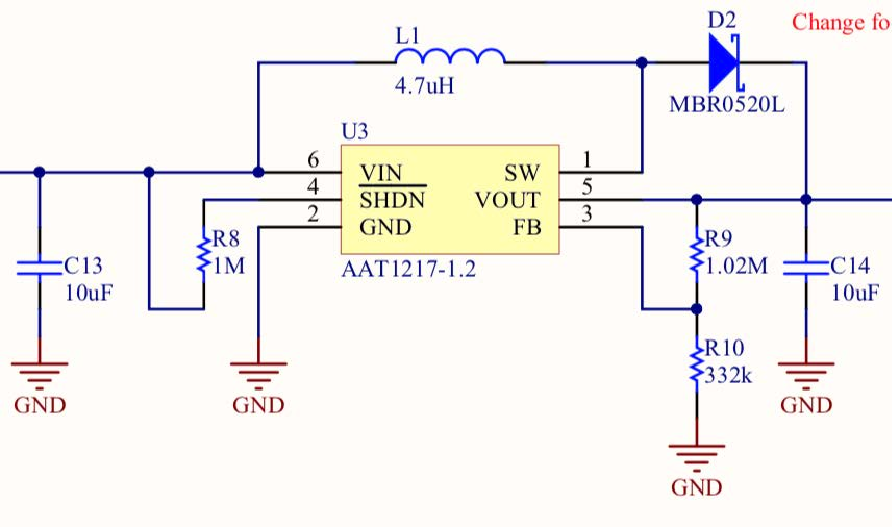
\includegraphics[height = 8cm]{figures/hardware/boost_schematic.pdf}
    \caption{Boost converter schematic excerpt.}
    \label{fig:boost}
\end{figure}
An external Schottky Diode is included since the output voltage exceeds \SI{4.5}{V}, and therefore the internal synchronous rectifier can no longer be used.
\\ \\
A high switching frequency was an important design parameter and was prioritized. Switched mode power supplies are inherently noisy, when the inductor is switched at the operating frequency the circuit will generate noise at the switching frequency and at harmonics of that frequency. This has the potential to radiate and interfere with the sensing circuit. Since the integrity of the state voltages of Cuk Converter is important for the performance of the converter.
\\ \\
To avoid interference, it was important that the Boost Converter operated at a fixed frequency that exceeded that of the \'Cuk Converter and also of the Nyquist rate of the ADC. Therefore, by choosing a boost converter that had a switching frequency that exceed that of the Anti-Aliasing filter ensured that the noise was not present in the sensed signals. The AAT1217 operates at a fixed frequency of 1.2MHz, this well exceeds the switching frequency of the \'Cuk converter.
\\ \\
Choosing the current rating of the boost converter was another important design constraint. This was a difficult specification to quantify as it varied with the input and output voltages of the converters.
\\ \\
A Boost converter topology was chosen as it allowed for the power to be stepped-up to a higher voltage will still being able to operate at the supply voltages. Due to the way that the charge controller (LTC4425) the ultra-capacitor stack will always be charged to slightly lower than the \SI{5}{V} output is specified. Hence the input to the boost converter will always be less than its fixed output of \SI{5}{V}.
%%%%%%%%%%%%%%%%%%%%%%%%%%%%%%%%%%%%%%%%%%%%%%%%%%%%%%%%%%%%%%%%%%%%%%%%%%%%%%%%

\subsubsection{Linear regulator}
Several devices, including the microcontroller require a nominal \SI{3.3}{V} to operate therefore a Linear Voltage Regulator was used to drop the 5V output from the boost converter down to \SI{3.3}{V}. The Microcontroller MCP1073A \SI{250}{mA}, \SI{16}{V}, Low Quiescent Current LDO Regulator was chosen.
\begin{figure}[H]
    \centering
    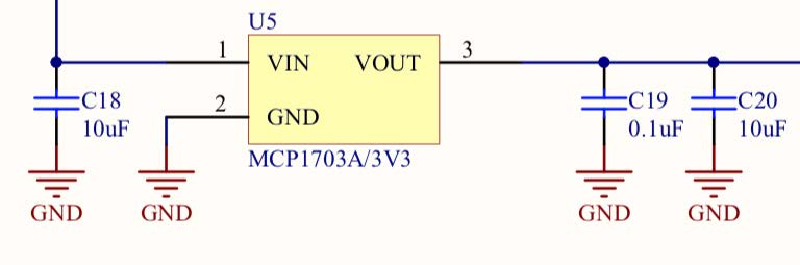
\includegraphics[width = 12cm]{figures/hardware/regulator_schematic.pdf}
    \caption{Linear regulator converter schematic excerpt.}
    \label{fig:regulator}
\end{figure}
To allow for flexibility in power supply design, the linear regulator was chosen such that it had a wide operating range. Allowing for a \SI{9}{V} DC supply to be used as a backup, in the event that USB charging option didn’t meet up performance criteria. The MCP1073A supports input voltages up to \SI{16}{V}. Additionally this allow the ultra-capacitors to be bypassed completely, allowing for operation directly was the \SI{9}{V} dc supply.

\paragraph{Power supply rejection ratio (PSRR) and output noise}
Since the \SI{3.3}{V} voltage rail would be used to supply the analog components of the system, this included the ADC and the op amps used to sense the input and output for the controller. As a switching power supply was used to maintain a constant \SI{5}{V} across most of its capacity, this supply rail was inherently noisy. To maintain a clean DC voltage on the supplies of these sensitive analog components it was important to consider the power supply rejection ratio of the LDO \cite{supply_ripple}.
\\ \\
The MCP1703A LDO Regulator has a PSRR below $-\SI{50}{dB}$ for frequencies above \SI{1}{MHz} (\SI{200}{mV} of ripple) \cite{mcp1703a}. As the switching frequency of the Boost Converter is typically \SI{1.2}{MHz} this will assist in producing a clean DC supply voltage for the analog circuitry.
%%%%%%%%%%%%%%%%%%%%%%%%%%%%%%%%%%%%%%%%%%%%%%%%%%%%%%%%%%%%%%%%%%%%%%%%%%%%%%%%
\subsubsection{Voltage inverter}
Since the \'Cuk Converter topology produces an inverted output the op amps used in the sensing circuitry must use dual supplies. The ADN8829 Switched-Capacitor Voltage Inverter is used in conjunction with the LDO regulator to produce $\pm\SI{3.3}{V}$ supply rails for the op amps.
\begin{figure}[H]
    \centering
    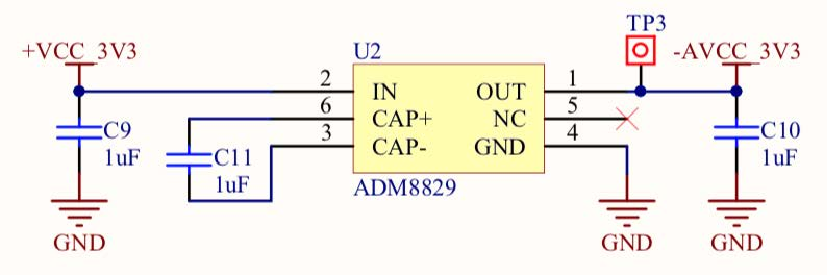
\includegraphics[width = 12cm]{figures/hardware/inverter_schematic.pdf}
    \caption{Voltage inverter schematic excerpt.}
    \label{fig:inverter}
\end{figure}
It was identified that a switched capacitor technique would be employed to generate the negative voltage as it was cost effective and had required little redesign to include. Due to a misunderstanding of the operation of the \'Cuk Converter, most of the hardware was designed before (including the sensing circuity) a negative supply was identified as a requirement. Therefore, the easy of integration was important to not delay the prototype further.
\\ \\
The ADM8829 was chosen as it was designed to be used for op amp supply rails and required minimal additional components. The recommended input and output capacitors were already included in the bill of materials, reducing design time. 
\\ \\
Switch capacitor converters, not unlike boost converters, are inherently noisy. By varying which terminal of the external capacitor is connected to ground periodically, a negative voltage is generated. This produces a significant ripple on the output which must be filtered to avoid corrupting the measurements made by the sensing circuitry. The Charge-Pump Frequency is typically \SI{120}{kHz}. This is close to the operating frequency of the \'Cuk Converter, consequently care must be take such that this does not interfere with the measures made by the sensing circuitry. Output ripple can vary between \SI{25}{mV} to \SI{130}{mV} peak-peak \cite{adm8829}, which when the sensed voltages are scaled by the resistive dividers will be of the same order of magnitude. In the next section the circuitry used to attenuate most of the ripple was outline. In future designs this particular chip would not be used and one with a much higher frequency would be used, however lost cost charge pump circuits in the MHz are rare. 
\\ \\
Produces \SI{25}{mA} of output current which is more than enough to supply the op amps. Include reference to calculations. However it is vital that the $-\SI{3.3}{V}$ power rail is not routed near any of the sense lines as this would interfere with the \'Cuk Converter which is switching at a similar frequency.
%%%%%%%%%%%%%%%%%%%%%%%%%%%%%%%%%%%%%%%%%%%%%%%%%%%%%%%%%%%%%%%%%%%%%%%%%%%%%%%%
%%%%%%%%%%%%%%%%%%%%%%%%%%%%%%%%%%%%%%%%%%%%%%%%%%%%%%%%%%%%%%%%%%%%%%%%%%%%%%%%
\newpage
\subsection{Gate driver}
\begin{figure}[H]
\centering
\fbox{
\begin{circuitikz}[scale = 0.75]
\draw (5,2)
	node[nmos](nmos1) {}
	(nmos1.G) node[right = 10mm]{NTD20N06}
	(nmos1.D) to (5,4)
	(nmos1.S) to (5,0);
\draw (-1,2) to [R, l_=$10 \ \mathsf{\Omega}$] (2,2) -- (nmos1.G);
\draw (2,2) -- (2,1) to [R, l_=$10 \ \mathsf{k\Omega}$] (5,1);
\draw (-1,2) node[ocirc, label=left:PWM] {};
\draw (5,4) node[ocirc, label=above:load] {};
\draw (5,0)	node[ground] {};
\end{circuitikz}
}
\caption{}
% \label{}
\end{figure}
MOSFETs were chosen as the switching component in the SMPS due to its increased power efficiency and rate of switching over a BJT. This increase in switching speed allowed for converter topologies that required smaller inductance and capacitance values, overall leading to smaller component sizes on the board. This was a serious design constraint, as to achieve the desired specifications, considerably large capacitance and inductance values were required. As outlined in section \ref{sec:ss_averaging} component values are inversely proportional to the switching frequency. Hence by choosing a large switching frequency we were able to obtain components that were both small and cost effective.
\\ \\
MOSFETs operate in a fundamentally different way to BJTs, this is in part due to the input impedance of both devices. A MOSFET is a voltage controller current source, and ideally the Gate of the MOSFET has large input impedance resulting in zero current draw. However, in practice the MOSFET gate acts as two separate capacitors, one between gate and drain and the other between gate and source. For the gate voltage to increase, the total input capacitance (sum of both the gate-drain and gate-source parasitic capacitances) must be charged. 
\\ \\
It is important to note that a MOSFET essentially dissipates not power when it either in the fully on or fully of states. The region in between, known as the transition region, is when the transistor dissipates most of its energy. Hence it is important that the time spent in this region in minimized.
\\ \\
%\textbf{discuss the fet that was used}
The output pin of a microcontroller is usually adequate to drive a small-signal logic level MOSFET. However, two issues arise when driving larger power MOSFETs that have been designed to deal with the higher current and voltages of power applications.
\begin{itemize}
    \item Increased gate/input capacitance. Due to the low current sink/source capabilities of microcontrollers, they are designed to only drive relatively small capacitive loads (in the order to 10-100pF). Power MOSFETs on the other hand can have input capacitances on the order of thousands of pico-farads.
    \item Higher gate/threshold voltage. Most power MOSFETs require voltages exceeding \SI{12}{V} to fully turn on. Therefore, a common TTL or CMOS logic signals of \SI{3.3}{V} or \SI{5}{V} is often not enough.
\end{itemize}
To maximize the switching frequency, such that the MOSFET spends the least amount of time in the transition state as possible, we must force a lot of charge into the gate very quickly. This, unsurprisingly, requires large peak currents.
\\ \\
%\textbf{Include calculations of peak gate currents required to attain the high switching speeds.}
%\\ \\
A gate capacitor is included in series with the gate of the transistor. Increasing the resistance resulted in the charging current being reduced, however it also slowed down the maximum switching speed. Reducing the current flow in the gate too much resulted in the gate charging slower than the speed it was switched, producing significant distortion of the waveform. 
\\ \\
Decreasing the gate resistor $R_g$ resulted in faster switching, however this produced larger current spikes in excess of $\pm\SI{300}{mA}$. This was simulated in LTSpice with the chosen MOSFET’s SPICE model.
\begin{itemize}
    \item Rise/fall time of a PWM signal produced by the MCU PWM module was minimum 5ns.
    \item \SI{10}{\ohm} have an appropriate response while limiting the instantaneous current, however it was still upwards of $\pm\SI{200}{mA}$.
    \item PWM frequency of \SI{250}{kHz}. Chosen to allow for flexibility in the design of the \'Cuk converter.
\end{itemize}
\SI{420}{\ohm} limits the gate current to under \SI{12}{mA} however this significantly distorted the PWM signal as the MOSFET is no longer driven to saturation during the switch on time. Hence a gate driver IC is required. See simulation results in \textbf{appendix ??} for detailed analysis. 
\\ \\
The Microchip TC4427A was chosen as the gate driver for the hardware implementation. It was chosen due to a number of features:
\begin{itemize}
    \item Non-inverting output meant that the control algorithm implemented on the microcontroller didn’t need to be altered in order for it to operate correctly.
    \item Wide Input Supply Voltage Operating Range (\SI{4.5}{V} to \SI{18}{V}). Allowed for a wide range of MOSFETs to be driven with the same chip.
    \item High Capacitive Load Drive Capability (\SI{1000}{pF}) and High Peak Output Current (\SI{1.5}{A}).
\end{itemize}
Finally, the TC4427A was included in the LTSpice model and produced an identical response. However, it can safely source and sink the required current. See appendix \ref{apx:sim_mosfet}.
\begin{figure}[H]
    \centering
    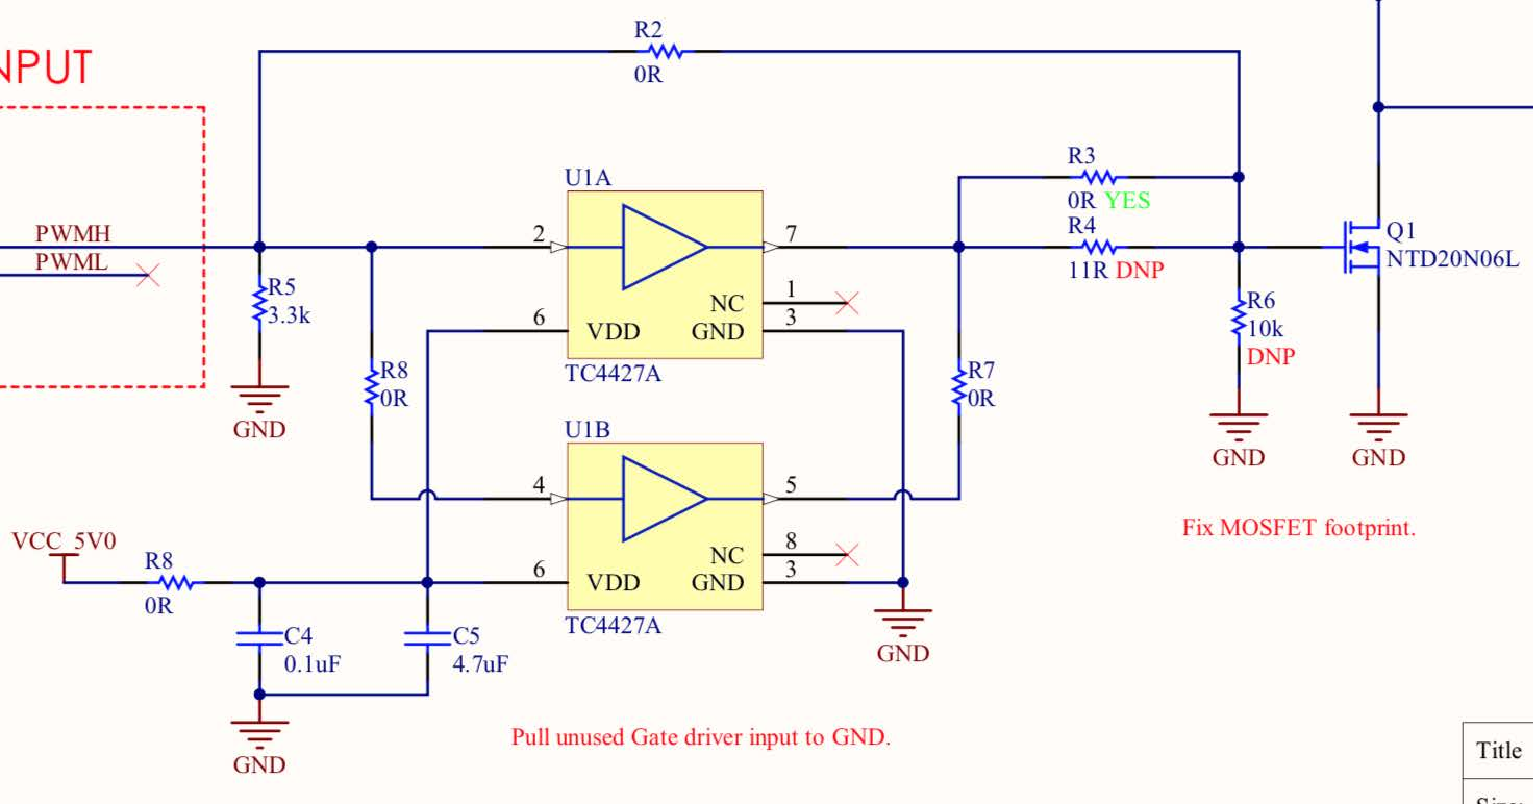
\includegraphics[height = 8cm]{figures/hardware/gate_driver_schematic.pdf}
    \caption{Gate driver schematic excerpt.}
    \label{fig:gate_driver}
\end{figure}
%%%%%%%%%%%%%%%%%%%%%%%%%%%%%%%%%%%%%%%%%%%%%%%%%%%%%%%%%%%%%%%%%%%%%%%%%%%%%%%%
\newpage
\subsection{Converter}
Using the components values outlined in section \ref{sec:control_ultimate} the \'Cuk Converter was implemented in hardware using discrete components.
\begin{figure}
\centering
    \fbox{
    % \includegraphics[height = 10cm]{figures/hardware/converter_schematic.PNG}
    % placeholder image - fix when have converter schematic
    
\includegraphics[width = 10cm]{figures/hardware/black.jpg}
    }
    \caption{\'Cuk converter schematic excerpt.}
    \label{fig:converter_schematic}
\end{figure}
%%%%%%%%%%%%%%%%%%%%%%%%%%%%%%%%%%%%%%%%%%%%%%%%%%%%%%%%%%%%%%%%%%%%%%%%%%%%%%%%
%%%%%%%%%%%%%%%%%%%%%%%%%%%%%%%%%%%%%%%%%%%%%%%%%%%%%%%%%%%%%%%%%%%%%%%%%%%%%%%%
\clearpage
\subsection{Ultimate system parameters}\label{sec:system_params}
\subsubsection{\'{C}uk converter}
\begin{table}[H]
\centering
\begin{tabular}{|c|c|c|}
\hline
% Designator & Value & ESR & Manufacturer part number\\
Designator & Value & ESR (if applicable)\\
\hline
$L_1$ & $470 \ \mathsf{\mu H}$ & $83.45 \ \mathsf{m \Omega}$\\
\hline
$L_2$ & $470 \ \mathsf{\mu H}$ & $83.45 \ \mathsf{m \Omega}$\\
\hline
$C_1$ & $24 \ \mathsf{\mu F}$ as $2 \times 12 \ \mathsf{\mu F}$ in parallel & $45 \ \mathsf{m \Omega}$ each\\
\hline
$C_2$ & $8.2 \ \mathsf{\mu F}$ & $80 \ \mathsf{m \Omega}$\\
\hline
$R_o$ & $36 \ \mathsf{m \Omega}$ & -\\
\hline
$R_D$ & $1.3 \ \mathsf{\Omega}$ & -\\
\hline
$V_D$ & $0.36 \ \mathsf{V}$ & -\\
\hline
$R$ & $100 \ \mathsf{\Omega}$ & -\\
\hline
\end{tabular}
\caption{}
\label{tab:cuk_values}
\end{table}
%%%%%%%%%%%%%%%%%%%%%%%%%%%%%%%%%%%%%%%%%%%%%%%%%%%%%%%%%%%%%%%%%%%%%%%%%%%%%%%%
\subsubsection{Peripherals}
%%%%%%%%%%%%%%%%%%%%%%%%%%%%%%%%%%%%%%%%%%%%%%%%%%%%%%%%%%%%%%%%%%%%%%%%%%%%%%%%
\subsubsection{Defining the operating point to linearise about}\label{sec:control_params}
\begin{table}[H]
\centering
\begin{tabular}{|c|c|c|}
\hline
Designator & Value\\
\hline
$V_g$ & $5 \ \mathsf{V}$\\
\hline
$V_D$ & $0.36 \ \mathsf{V}$\\
\hline
$D$ & $50 \ \mathsf{\%}$\\
\hline
\end{tabular}
\caption{}
\label{tab:control_values}
\end{table}
%%%%%%%%%%%%%%%%%%%%%%%%%%%%%%%%%%%%%%%%%%%%%%%%%%%%%%%%%%%%%%%%%%%%%%%%%%%%%%%%
\subsubsection{Other system parameters}\label{sec:system_params_other}
\begin{table}[H]
\centering
\begin{tabular}{|c|c|c|}
\hline
% Designator & Value & ESR & Manufacturer part number\\
Designator & Value\\
\hline
$f_\text{switching}$ & $100 \ \mathsf{kHz}$\\
\hline
$f_\text{sample}$ & $4 \ \mathsf{kHz}$\\
\hline
$d \text{(min)}$ & $0 \ \mathsf{\%}$\\
\hline
$d \text{(max)}$ & $90 \ \mathsf{\%}$\\
\hline
\end{tabular}
\caption{}
\label{tab:system_values}
\end{table}
% Note that $D$ denotes the duty ratio used in state-space averaging as the operating point about which the system is linearised.
%%%%%%%%%%%%%%%%%%%%%%%%%%%%%%%%%%%%%%%%%%%%%%%%%%%%%%%%%%%%%%%%%%%%%%%%%%%%%%%%
%%%%%%%%%%%%%%%%%%%%%%%%%%%%%%%%%%%%%%%%%%%%%%%%%%%%%%%%%%%%%%%%%%%%%%%%%%%%%%%%